% fig_rotating_mode.tex - EM field pattern visualization (top view)
% Standalone compilation: pdflatex fig_rotating_mode.tex
\documentclass[tikz,border=5pt]{standalone}
\usepackage{tikz}
\usepackage{amsmath}
\usetikzlibrary{decorations.markings,arrows.meta,calc}

\begin{document}
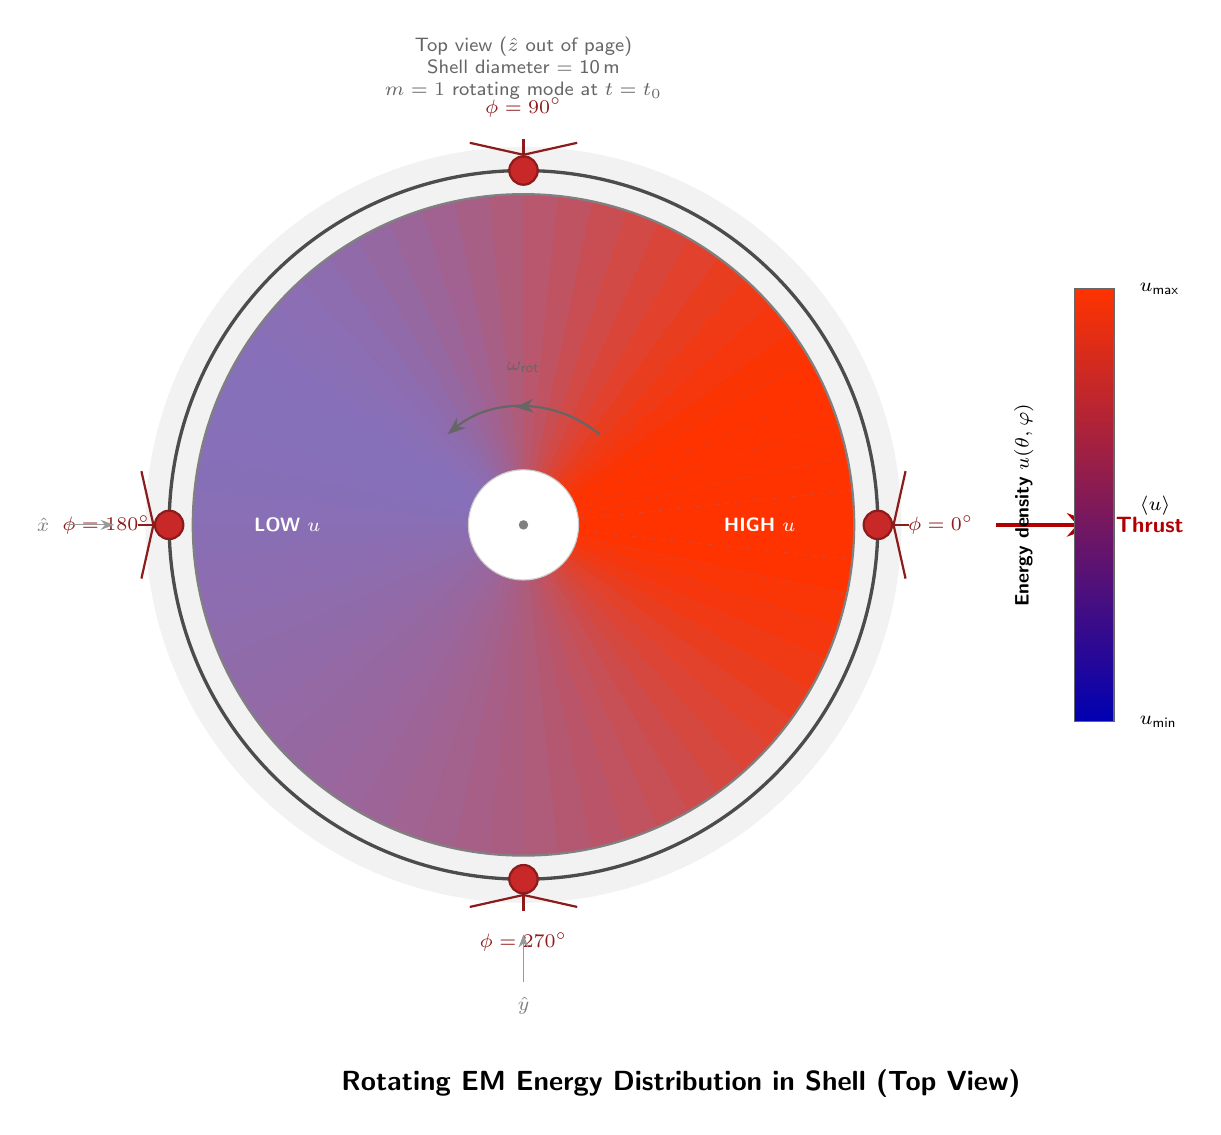
\begin{tikzpicture}[
    >=Stealth,
    every node/.style={font=\footnotesize\sffamily},
]

\definecolor{feedRed}{RGB}{200,40,40}

\def\R{4.5}  % shell radius (top view)

% Background disk
\fill[black!5] (0,0) circle (\R+0.3);

% --- Energy density color map (asymmetric, rotating) ---
% Discretized into angular sectors using blue->red gradient via opacity trick
% Thrust side (0 deg) is hot/red; opposite (180 deg) is cool/blue

% Base layers: blue everywhere, then red with angle-dependent opacity
\fill[blue!70!black, opacity=0.5] (0,0) circle ({\R-0.3});
\fill[white] (0,0) circle (0.7);

% Red overlay sectors: opacity ~ cos(angle) for asymmetric energy
\foreach \a in {0,6,...,354} {
    \pgfmathsetmacro{\anext}{\a+6}
    \pgfmathsetmacro{\opval}{max(0.02, 0.5 + 0.45*cos(\a) + 0.1*cos(2*\a - 30))}
    \fill[red!80!yellow, opacity=\opval]
        ({\a}:0.7) -- ({\a}:{\R-0.3})
        arc ({\a}:{\anext}:{\R-0.3})
        -- ({\anext}:0.7)
        arc ({\anext}:{\a}:0.7) -- cycle;
}

% Shell ring
\draw[black!70, very thick] (0,0) circle (\R);
\draw[black!50, thick] (0,0) circle ({\R-0.3});
\draw[black!20, thin] (0,0) circle (0.7);

% ============================================================
% FEED POINTS (4 locations, 90 deg apart)
% ============================================================
\foreach \a/\phase in {0/0, 90/90, 180/180, 270/270} {
    \fill[feedRed] ({\a}:\R) circle (0.18);
    \draw[feedRed!70!black, thick] ({\a}:\R) circle (0.18);
    \node[font=\scriptsize\sffamily, feedRed!70!black] at ({\a}:{\R+0.8}) {$\phi=\phase^\circ$};
}

% Feed point symbols
\foreach \a in {0,90,180,270} {
    \draw[feedRed!70!black, thick]
        ({\a}:{\R+0.2}) -- ({\a}:{\R+0.4});
    \draw[feedRed!70!black, thick]
        ({(\a)-8}:{\R+0.4}) -- ({\a}:{\R+0.2}) -- ({(\a)+8}:{\R+0.4});
}

% ============================================================
% ASYMMETRY INDICATION
% ============================================================
\draw[-{Stealth[length=4mm,width=3mm]}, red!70!black, very thick]
    ({\R+1.5},0) -- ({\R+2.8},0);
\node[red!70!black, font=\footnotesize\sffamily\bfseries, right] at ({\R+2.9},0)
    {Thrust};

\node[white, font=\scriptsize\sffamily\bfseries] at (3,0) {HIGH $u$};
\node[white, font=\scriptsize\sffamily\bfseries] at (-3,0) {LOW $u$};

% ============================================================
% ROTATION ARROW
% ============================================================
\draw[->, black!60, thick,
      decoration={markings, mark=at position 0.55 with {\arrow{>}}},
      postaction={decorate}]
    (50:1.5) arc (50:130:1.5);
\node[black!60, font=\scriptsize\sffamily] at (90:2.0) {$\omega_\text{rot}$};

% Coordinate labels
\draw[->, black!40, thin] (-5.8,0) -- (-5.2,0);
\node[black!50, font=\scriptsize\sffamily] at (-6.1,0) {$\hat{x}$};
\draw[->, black!40, thin] (0,-5.8) -- (0,-5.2);
\node[black!50, font=\scriptsize\sffamily] at (0,-6.1) {$\hat{y}$};

% Center mark
\fill[black!50] (0,0) circle (0.06);

% ============================================================
% COLOR BAR
% ============================================================
\begin{scope}[xshift=7cm, yshift=-2.5cm]
    % Blue to red gradient bar
    \shade[bottom color=blue!70!black, top color=red!80!yellow]
        (0,0) rectangle (0.5,5.5);
    \draw[black!60, thin] (0,0) rectangle (0.5,5.5);
    \node[font=\scriptsize\sffamily, anchor=west] at (0.7,0) {$u_\text{min}$};
    \node[font=\scriptsize\sffamily, anchor=west] at (0.7,5.5) {$u_\text{max}$};
    \node[font=\scriptsize\sffamily, anchor=west] at (0.7,2.75) {$\langle u \rangle$};
    \node[font=\scriptsize\sffamily\bfseries, anchor=south, rotate=90] at (-0.4,2.75)
        {Energy density $u(\theta,\varphi)$};
\end{scope}

% ============================================================
% ANNOTATIONS
% ============================================================
\node[font=\scriptsize\sffamily, align=center, black!60] at (0,5.8)
    {Top view ($\hat{z}$ out of page)\\
     Shell diameter = 10\,m\\
     $m=1$ rotating mode at $t=t_0$};

% ============================================================
% TITLE
% ============================================================
\node[font=\normalsize\sffamily\bfseries, anchor=north] at (2,-6.8)
    {Rotating EM Energy Distribution in Shell (Top View)};

\end{tikzpicture}
\end{document}
